%!TEX root = umthsmpl.tex
\chapter{Difficulty Estimation}
\label{difficulty-estimation}

Developers have resorted to adhoc methods for updating the difficulty in many blockchain systems. So far, there has been no previous work on analyzing the efficiency and correctness of these methods. In fact, because some blockchain systems do not accurately update difficulty, networks see enormous variance in inter-block delay. If mining power were constant in these networks, then difficulty could be kept constant. However, as seen with many blockchain systems, including a recent example with Bitcoin Cash, mining power fluctuates within these networks, requiring a readjustment of network parameters, including difficulty. Therefore, in this chapter, we use the most prominent cryptocurrency, Bitcoin Core, as a testbed for analyzing difficulty, and then propose alternative methods that could potentially increase efficiency. 

\section{Proof-of-work in Blockchain Systems}
Bitcoin Core uses a simple POW algorithm based on cryptographic
hashing, proposed earlier by Douceur~\cite{Douceur:2002}.
Specifically, miners apply a 256-bit cryptographic hash algorithm~\cite{hashcash} to
an 80-byte {\em block header}, and the puzzle is solved if the
resulting value is less than a known {\em target}, $0<t<2^{256}$. The
header in Bitcoin Core consists of the Merkle root of the set of
transactions, a timestamp, the target (stored as $2^{224}/t$), a {\em
  nonce}, and the hash of the prior block's header. If the hash is not
less than the target, then a new nonce is selected to generate a new
hash (the Merkle root can be adjusted as well). This process repeats
until some miner finds a solution.
  
Each time a nonce is selected and the block
header is hashed, the miner is sampling a value from a discrete uniform
distribution with range $[0,2^{256}-1]$. The probability of solving the POW and
discovering a block is the cumulative probability of selecting a value
from $[0,t]$, which is $t/{2^{256}}$. Hence, in expectation, the
number of samples needed to discover a block is ${2^{256}/t}$. Bitcoin Core
adjusts the target so that on average it takes about 600 minutes to
find a block. Typically, the target is described for convenience as a
{\em difficulty}, defined to be $D=2^{224}/t$. Bitcoin Core's difficulty
is set once every two weeks.

\para{Ethereum.} Ethereum operates very similarly to Bitcoin Core. Miners solve a POW problem that is more complicated
than Bitcoin Core in an attempt to disadvantage miners with custom ASICs.
However, in the end, a miner still compares a hash value to the target.
Specifically, the number of values in the block header is larger,
resulting in a 508-byte header. It's not the hash of the header that
is compared against the target, but the hash resulting from an
Ethereum-specific algorithm called ETHASH~\cite{ETHASH}, for which the
hash of the block header is the primary input. In the end, the POW
hash value is a sample from a discrete uniform distribution with range
$[0,2^{256}-1]$, and the probability of block discovery is
${t/2^{256}}$.

A major difference of Ethereum is that the target is set such that the
expected time between blocks is 15 seconds. This setting results
in quicker confirmation times, but as a result, the probability that two
miners announce blocks within the propagation time of a block
announcement is much higher. Therefore, there are many abandoned
forks in the chain. Ethereum uses a modified version of the GHOST~\cite{Sompolinsky:2015}
protocol for selecting the main fork of the blockchain: the main chain
follows the block at each level with the most POW on its subtree.
These differences do not affect the application of our algorithms; in
fact, the presence of abandoned forks is additional data which improves our
estimates.

%%%%%%%%%%%%%%%%%%%%%%%%%%%%%%%%%%%%%%%%
%\section{Problem Statement}
%Developers have resorted to adhoc methods for updating the difficulty in many blockchain systems. So far, there has been no previous work on analyzing the efficiency and correctness of these methods. In fact, because some blockchain systems do not accurately update difficulty, networks see enormous variance in inter-block delay. If mining power were constant in these networks, then difficulty could be kept constant. However, as seen with many blockchain systems, including a recent example with Bitcoin Cash, mining power fluctuates within these networks, requiring a readjustment of network parameters, including difficulty. Therefore, in this chapter, we use the most prominent cryptocurrency, Bitcoin Core, as a testbed for analyzing difficulty, and then propose alternative methods that could potentially increase efficiency. 

%%%%%%%%%%%%%%%%%%%%%%%%%%%%%%%%%%%%%%%%
\section{Preliminary Work}
In the following section, we describe Bitcoin Core's algorithm for setting difficulty and analyze its statistical properties. Then we describe an alternative estimator and compute the same set of statistical properties for comparison.
\subsection{Analysis of Bitcoin Core's Difficulty Estimation}
\para{Algorithm for setting difficulty.} Bitcoin Core's networks parameters are set such that a block is discovered every 10 minutes. Initially, difficulty starts at 1, and then for every 2016 blocks that are found, the timestamps of the blocks are compared to compute the time it took to find 2016 blocks. Let $t$ denote the time in minutes it took to find 2016 blocks. Because the network is configured such that 2016 blocks must take 2 weeks (20160 minutes), the old difficulty is multiplied by $20160 / t$. If the correction factor is greater than $4$ or less than $1/4$, then $4$ or $1/4$ are used, respectively, to prevent the change from being too abrupt.
\par \noindent Bitcoin Core's target and difficulty are related to each other as follows:
\begin{align}
\texttt{target} = \frac{\texttt{targetmax}}{\texttt{difficulty}} = \frac{2^{224}}{{D_i}},
\end{align} 
where $D_i$ is the $i$th time the difficulty is set~\cite{bitcoin:difficulty} and \texttt{targetmax} is the maximum value for the target. This equation shows us that the difficulty and target are inversely proportional: when difficulty increases, the target decreases. Therefore, a smaller target makes block creation more difficult, and as the difficulty goes up, so does the expected time needed to create a block. Next, we use concepts from queuing theory to compute the expected value and variance of Bitcoin Core's difficulty algorithm.

\para{Analysis of difficulty adjustment.}
Let $D_i$ denote the $i$th time the difficulty is set, and $X_k$ denote the number of minutes it took to generate the $k$th block after $D_i$ is set. 
%Using Bitcoin Core's algorithm, difficulty for the $i+1$st time is
%\begin{align}
%D_{i+1} &=D_i \frac{10n}{ \sum_{k=1}^n X_k}.
%%&= 10n^i \frac{1}{\prod_{x=0}^i t_x}
%\end{align}
%Let D be a sequence generated by the last equation where the first element of the sequence is $D_0 = 1$. 
Mining is an example of a Poisson process because under constant
mining power, blocks are mined continuously and independently at a
constant average rate.  Therefore, $X_k \sim$ \texttt{Exp}$(\beta)$ with $\beta = 1/\lambda$, assuming a fixed hash rate for the 2-week period after $D_i$ is set. In this parametrization of the Exponential, $\beta$ represents the survival parameter, and hence, the ratio describing the {\em expected time} it takes for one block to arrive. For example, ideally in Bitcoin Core $\beta=1/10$ minutes and in Ethereum $\beta=1/15$ seconds. Using Bitcoin Core's algorithm, the difficulty for the $i+1$st time given $D_i$ and $X_1, \dots, X_n$, where $n=2016$, is defined as
\begin{align}
D_{i+1} &= 10nD_i \Bigg(\frac{1}{\sum_{k=1}^{n} X_k}\Bigg).\label{eq:original-Bitcoin Core}
%&= 10n D_i \frac{1}{Y}
\end{align}
Next, we compute the expected value and variance of the difficulty each time it is set by Bitcoin Core's algorithm.

\para{Expected value of difficulty.}
Let D be a sequence generated by Equation~\ref{eq:original-Bitcoin Core} where the first element of the sequence is $D_0 = 1$. We can talk about the expected value of a term in sequence D, given its preceding term and the new data we see. 
\begin{align}
\EX[D_{i+1} | D_{i}, X_1, \dots, X_{n}] &= \EX\bigg[10n D_i \frac{1}{\sum_{k=1}^{n} X_k}\bigg] \\
&= 10n D_i \EX\bigg[\frac{1}{\sum_{k=1}^{n} X_k}\bigg] \\
&= 10n D_i \Bigg(\frac{1}{\beta(n-1)}\Bigg) \\
&= \frac{10n D_i}{\beta(n-1)}.
\end{align}
The sum of any number of exponential random variables is a gamma distribution, and Equation 2.5 can be obtained from Equation 2.4 using the definition of the expected value of an inverse gamma distribution.
%Refer to \url{https://stats.stackexchange.com/questions/139467/expected-value-of-y-1-x-where-x-sim-gamma} for proof. 

\para{Variance of difficulty.}
Additionally, we can also talk about the variance of a term in sequence D, given its preceding term and the new data we see. 
\begin{align}
\text{Var}(D_{i+1} | D_{i}, X_1, \dots, X_{n}) &= \text{Var}\bigg(10n D_i \frac{1}{\sum_{k=1}^{n} X_k}\bigg) \\
&= (10n D_i)^2 \text{Var}\bigg(\frac{1}{\sum_{k=1}^{n} X_k}\bigg) \\ 
&= (10n D_i)^2 \Bigg(\frac{1}{\beta^2(n-1)^2(n-2)}\Bigg) \\
&= \frac{(10n D_i)^2}{\beta^2(n-1)^2(n-2)}.
\end{align}
Once again, the sum of exponential random variables is a gamma distribution, and Equation 2.9 can be obtained from Equation 2.8 using the definition of variance for an inverse gamma distribution.
%Refer to \url{https://www.johndcook.com/inverse_gamma.pdf} and \url{https://ocw.mit.edu/courses/mathematics/18-443-statistics-for-applications-fall-2006/lecture-notes/lecture6.pdf} for explanation.

Next, we compute the bias and mean squared error (MSE) associated with Bitcoin Core's difficulty algorithm. However, in order to compute bias, we need the true underlying difficulty of the network. Therefore, we first explain how to compute the network's hash rate which we use to adjust difficulty correctly. This difficulty is then used for the calculation of bias and MSE, two statistical properties which we will compare with those of an alternative estimator. \\
\para{The relationship between hash rate and $\boldsymbol{\beta}$.}
Given difficulty $D_i$, the expected number of hashes, $h$, needed to meet the target for a block is
\begin{align}
\EX[h] =  \frac{2^{256}-1}{T_i} = \frac{2^{256}-1}{\sfrac{2^{224}}{D_i}} = \frac{D_i(2^{256}-1)}{2^{224}}, 
\end{align}
where $T_i$ is the target set for the $i$th time. Note that $\EX[h]$ describes the \textit{total} number of expected hashes needed to discover a block, and we have observations regarding the \textit{time} it takes to generate a block. Let $r$ be the hash rate of the network in minutes (i.e. the number of hashes per time unit), and X be a random variable describing the inter-arrival of blocks such that $X = X_1, \dots, X_{n}$, where $X \sim$ \texttt{Exp}$(\beta)$, with $\beta = 1/\lambda$/ The expected number of hashes for a block discovery is described by $r/\beta$.
\begin{align}
\EX[h] &= r \frac{1}{\beta}  \\
r &= \EX[h] \beta.
\end{align}

\para{Adjusting difficulty correctly.}
For Bitcoin Core, where the network is expected to solve a block every 10 minutes, the target for the $i+1$th time is adjusted as follows 
\begin{align}
\frac{(2^{256}-1)}{T_{i+1}} &= 10r \\
\frac{(2^{256}-1)}{T_{i+1}} &= 10\EX[h] \beta \\
\frac{(2^{256}-1)}{T_{i+1}} &= 10\frac{(2^{256}-1)}{T_i}\beta .
\end{align}
We rearrange Equation 2.16 to solve for $T_{i+1}$.
\begin{align}
T_{i+1} &= \frac{T_i}{10\beta}.
\end{align}
Substituting $T_i$ and $T_{i+1}$ with its definition using $D_i$ and $D_{i+1}$, respectively, is
\begin{align}
\frac{2^{224}}{D_{i+1}} &= \frac{\sfrac{2^{224}}{D_i}}{10\beta}.
%&= \frac{2^{224}}{T_{i+1}} \\
%&= \frac{2^{224}10\beta}{T_i} \\
%&= \frac{2^{224}10\beta}{\sfrac{2^{224}}{D_i}} \\
%D_{i+1} &= 10\beta D_i.
\end{align}
Then we solve for difficulty for the $i+1$th time as follows 
\begin{align}
%\frac{2^{224}}{D_{i+1}} &= \frac{\sfrac{2^{224}}{D_i}}{10\beta} \\
%&= \frac{2^{224}}{T_{i+1}} \\
%&= \frac{2^{224}10\beta}{T_i} \\
%&= \frac{2^{224}10\beta}{\sfrac{2^{224}}{D_i}} \\
D_{i+1}\frac{2^{224}}{D_i} &= 2^{224}10\beta \\
D_{i+1} &= 10\beta D_i.
\end{align}

\noindent Using Equation 2.20, we calculate the bias and MSE of Bitcoin Core's algorithm for setting difficulty. \\
\para{Bias of difficulty.}
\begin{align}
\text{bias}(D_{i+1}|D_i,X_1,...,X_n) &= \EX[D_{i+1}|D_i,X_1,...,X_n] - D_{i+1} \\
&= \frac{10n D_i}{\beta(n-1)} - 10\beta D_i.
%&= 10D_i \Bigg(\frac{n}{\beta(n-1)} - \beta \Bigg)
\end{align}

\para{MSE of difficulty.}
\begin{align}
\text{MSE}(D_{i+1}|D_i,X_1,...,X_n) &= \text{bias}(D_{i+1}|D_i,X_1,...,X_n)^2 + \text{Var}(D_{i+1}|D_i,X_1,...,X_n) \\
&= \Bigg(\frac{10n D_i}{\beta(n-1)} - 10\beta D_i\Bigg)^2 + \frac{(10n D_i)^2}{\beta^2(n-1)^2(n-2)}.
%&= \Bigg[10D_i \Bigg(\frac{n}{\beta(n-1)} - \beta \Bigg)\Bigg]^2 + \\
%&= (10D_i)^2 \Bigg(\frac{n^2}{\beta^2(n-1)^2} - \beta^2 - \frac{2\beta n}{\beta(n-1)} \Bigg) + \frac{(10n D_i)^2}{\beta^2(n-1)^2(n-2)}
\end{align}

%%%%%%%%%%%%%%%%%%%%%%%%%%%%%%%%%%%%%%%%
\subsection{Alternative Time Based Estimation}\label{sec:time based}
Now we propose an alternative estimator and show that it has lower variance, bias and MSE.
%In this section, we describe two blockchain-only methods of estimating
%miner hash rates. 
%%For these estimators, we treat the entire network as a single miner and a block as a status report 
%%that can only be observed at certain intervals. 
%Although these approaches have no additional network costs and do not require cooperation from miners, they are less accurate than status reports.  We then extend our techniques to allow for hash rate estimation of an individual or a subset of miners. As we show, this extension allows for the incremental deployment of status reports. 

%We would like to estimate the network hash rate, $\hat{h}$, using only
%the \emph{inter-arrival time} of mined blocks. 

\para{Estimator for $\boldsymbol{\beta}$, the expected inter-arrival time between blocks.} Let $X = X_1, \ldots, X_n$ denote the inter-arrival time between $n+1$ consecutive blocks on the blockchain. Given a consecutive sequence of $n+1$ blocks, $n$ inter-arrival times can be computed by subtracting the timestamp of each block from that of its preceding block. Note that $X \sim$ \texttt{Exp}$(\beta)$ with $\beta = 1/\lambda$, similar to the definition in the previous section. It it well known that the unbiased MLE estimator, $\hat{\beta}$, for $\beta$ is
\begin{align}
\hat{\beta} = \frac{\sum_{k=1}^{n} X_i}{n}. \label{eq:beta-hat}
\end{align}

\para{Adjusting difficulty.}
Using our estimate of $\beta$, we can adjust the difficulty for the $i+1$th time as follows 
\begin{align}
%\frac{D_{i+1}(2^{256}-1)}{2^{224}} &= 10r \\
%\frac{D_{i+1}(2^{256}-1)}{2^{224}} &= \frac{10D_i(2^{256}-1)\hat{\beta}}{2^{224}} \\
D_{i+1} &= 10 D_i \hat{\beta}.
\end{align}

\noindent Next, we compute the expected value, variance, bias and MSE associated with this new estimator. \\
\para{Expected Value of New Difficulty.}
\begin{align}
\EX[D_{i+1} | D_{i}, X_1, \dots, X_{n}] &= \EX[10 D_i \hat{\beta}] \\
&= 10 D_i \EX[\hat{\beta}] \\
&= 10 D_i\beta.
\end{align}

\para{Variance of New Difficulty.}
\begin{align}
\text{Var}(D_{i+1} | D_{i}, X_1, \dots, X_{n}) &= \text{Var}(10 D_i \hat{\beta}) \\
&= (10 D_i)^2 \text{Var}(\hat{\beta}) \\
&= \frac{(10 D_i\beta)^2}{n}.
\end{align}

\para{Bias of New Difficulty.}
\begin{align}
\text{bias}(D_{i+1}|D_i,X_1,...,X_n) &= \EX[D_{i+1}|D_i,X_1,...,X_n] - D_{i+1} \\
&= 10 D_i\beta - 10 D_i\beta \\
&= 0.
\end{align}

\para{MSE of New Difficulty.}
\begin{align}
\text{MSE}(D_{i+1}|D_i,X_1,...,X_n) &= \text{bias}(D_{i+1}|D_i,X_1,...,X_n)^2 + \text{Var}(D_{i+1}|D_i,X_1,...,X_n) \\
&= \frac{(10 D_i\beta)^2}{n}.
\end{align}

%%%%%%%%%%%%%%%%%%%%%%%%%%%%%%%%%%%%%%%%
\subsection{Comparison of Estimators}
Note that our alternative estimator has zero bias compared to Bitcoin Core's original estimator. Additionally, under the appropriate constraints, variance and MSE are also significantly lower.
\par \noindent \para{Variance.}
\begin{align}
\frac{(10 D_i\beta)^2}{n} \leq \frac{(10n D_i)^2}{\beta^2(n-1)^2(n-2)} \\
\frac{\beta^2}{n} \leq \frac{n^2}{\beta^2(n-1)^2(n-2)} 
\end{align}
Our estimator (LHS) has lower variance than the original estimator (RHS) for $n>2$ and $0<\beta<1$.
%Reduce[\frac{\beta^2}{n} \leq \frac{n^2}{\beta^2(n-1)^2(n-2)}, \beta<1]

\para{MSE.}
\begin{align}
\frac{(10 D_i\beta)^2}{n} \leq \Bigg(\frac{10n D_i}{\beta(n-1)} - 10\beta D_i\Bigg)^2 + \frac{(10n D_i)^2}{\beta^2(n-1)^2(n-2)}
\end{align}
Our estimator (LHS) has lower variance than the original estimator (RHS) for $n>2$, $0<\beta<1$ and $D_i \in \mathcal{R}$. \reminder{Add figure for Bitcoin Core, Litecoin, Ethereum, Bitcoin Core Cash, Ripple. After 2016 blocks generated, Litecoin will adjust difficulty to estimated difficulty in order to keep the block generation time at 150 seconds. Bitcoin Core cash has a window of only 144 blocks. and uses a sliding window. Ethereum uses 1 block, can't find ripple}

%Reduce[\frac{(10 D \beta)^2}{n} \leq \Bigg(\frac{10n D}{\beta(n-1)} - 10 \beta D\Bigg)^2 + \frac{(10n D)^2}{\beta^2(n-1)^2(n-2)}, \beta<1]
%So, time based estimator is indeed better.

%%%%%%%%%%%%%%%%%%%%%%%%%%%%%%%%%%%%%%%%
\section{Proposed Work} \label{section:difficulty-proposed-work}
In this section, we introduce \textit{status reports} that are to be used for a second estimator, and then proposed work relating to this chapter.

\subsection{Status Reports}
Attackers can easily lie about the timestamps on the blocks with our new time based estimator. Therefore, an alternative estimator we plan to develop uses status reports, which is a block header except that the POW does not satisfy the current target. Every $\alpha$ minutes, a parameter determined by the network, the miners send periodic status reports that include the minimum hash value, which represents the hash found since the last block broadcast on the chain. To be clear, each status report does not directly report the minimum hash value; instead, reports are of the input values to the POW algorithm. Because attackers can't lie about their POW, an estimator based on the minimum hash value is safer and can be used to adjust the emergency difficulty when the network fails to produce a block for an unusually long time. We plan to compute the the variance and MSE of the status report based estimator, and compare its performance with other methods.

\subsection{Key Questions}
We were able to show that our time based estimator performs better than Bitcoin Core's unjustified method. To extend this chapter, we propose to answer the following questions centered around a few key themes:
\begin{enumerate}
\item \textbf{Analysis of attacks against our estimators.} What happens when the timestamps on the blocks are reported inaccurately by an attacker? How much error can an attacker introduce?
\item \textbf{Security bounds of the estimators.} What are the Chernoff bounds associated with our estimators?
\item \textbf{Settings of network parameters and their consequences.} How often should difficulty be adjusted? How often should miners send status reports? Should non-overlapping windows of blocks be used to compute difficulty at each iteration? Should there be some overlap of blocks between windows at each iteration?
\item \textbf{Individual parameter settings for peers.} Given a required error rate, what is the shortest window of time (or number of blocks) needed to estimate difficulty correctly?
\item \textbf{Fluctuations in mining power.} Given that mining power is changing, how quickly can either estimator adapt to change?
\item \textbf{Pros and cons of our estimators.} What are the advantages and disadvantages of status reports compared to the time based estimator? For example, the status report based estimator uses the minimum hash value, which is arguably safer because miners have to show their POW. On the other hand, for the time based estimator, there is no POW required when reporting timestamps.
\end{enumerate}

%\paragraph*{Overview}

%\begin{equation}
%\arg\max_\mathbf{s} p(\mathbf{s}|u).
%\end{equation}
%
%\begin{figure}\begin{center}
%		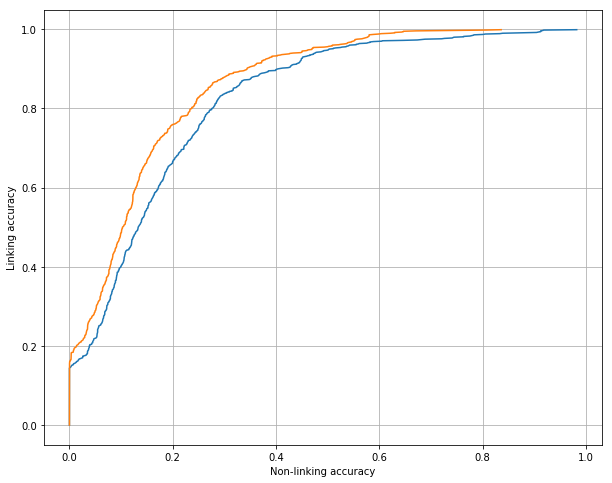
\includegraphics[width=0.7\textwidth]{graphics/linking2}
%		\caption{The $x$-axis represents accuracy of identifying a set of traces unlinked, and the $y$-axis represents the accuracy of the same set linked based on Equation~\ref{eq:link3}. Red is a link before, and blue is a link after.
%		\label{fig:linkcdf}}
%\end{center}\end{figure}